Let $\text{E}_b = \{ x \in \mathbb{R}^2 | (\mathbf{x} - \mathbf{\mu})^T \Sigma^{-1}(\mathbf{x} - \mathbf{\mu}) = b \}$ be the ellipsoid shown in the figure, which is centered in $\mathbf{\mu} = \text{E}[X] = [0 \quad 2]^T$. Applying Theorem 2.7 in Härdle and Simar, we can determine that the principal axes of $\text{E}_b$ will be in the direction of the eigenvectors of $\Sigma^{-1}$ and that their half-lengths will be given by $\sqrt{\frac{b}{\lambda_i}}$, $i =1,2$ where $\lambda_i$ are the eigenvalues of $\Sigma^{-1}$.

We know that $\Sigma$ and $\Sigma^{-1}$ share the same eigenvectors and that the eigenvalues of $\Sigma^{-1}$ are  $\Tilde{\lambda_i}= \frac{1}{{\lambda_i}}$ where $\lambda_i$ are the eigenvalues of $\Sigma$. 
Thus, the principal axes of $\text{E}_b$ lie along $[\: 1 \;  1\: ]^T$ and $[\: 1 \ -1\:]^T$, and the lengths of the half-lengths are $d_1 = \sqrt{2b} \approx 3.03$ and $d_2 =  \sqrt{4b} \approx 4.29$.
%%%jeg lurer på om det burde vært b^2 i ligningen for ellipsen? og vi må lage figur her og legge inn, derfor jeg har brukt navn d1 og d2


$(\mathbf{x}- \mathbf{\mu})^T\Sigma^{-1} (\mathbf{x}- \mathbf{\mu})$ defines a distance from the centre $\mathbf{\mu}$, so that for all points $\mathbf{x} \in \text{E}_b$, $\mathbf{x} \leq b$. 
Using the Mahalanobis transformation, we recognize that 
\begin{equation*}
    (\mathbf{x}- \mathbf{\mu})^T\Sigma^{-1} (\mathbf{x}- \mathbf{\mu})
    = (\mathbf{x}- \mathbf{\mu})^T(\Sigma^{-1/2})^T\Sigma^{-1/2}(\mathbf{x}- \mathbf{\mu}) = Z^TZ = \sum_{i=1}^p z_i^2
\end{equation*}

where $Z \sim N(\mathbf{0}, \sigma^2 I)$ so that $z_i \sim N(0,\sigma^2)$ and $z_i^2 \sim \mathcal{X}_1^2$. As a sum of p $\mathcal{X}_1^2$ variables, $(\mathbf{x}- \mathbf{\mu})^T\Sigma^{-1} (\mathbf{x}- \mathbf{\mu})$ is thus $\mathcal{X}_p^2$ distributed with $\text{p}=2$. %%må noe av dette vises? idk

Accordingly, the probability that $\mathbf{X}$ falls within the given ellipse is given by the chi-squared distribution, $\text{P}(\mathbf{X} \leq 4.6) = 0.9$.


\begin{figure}
    \centering
    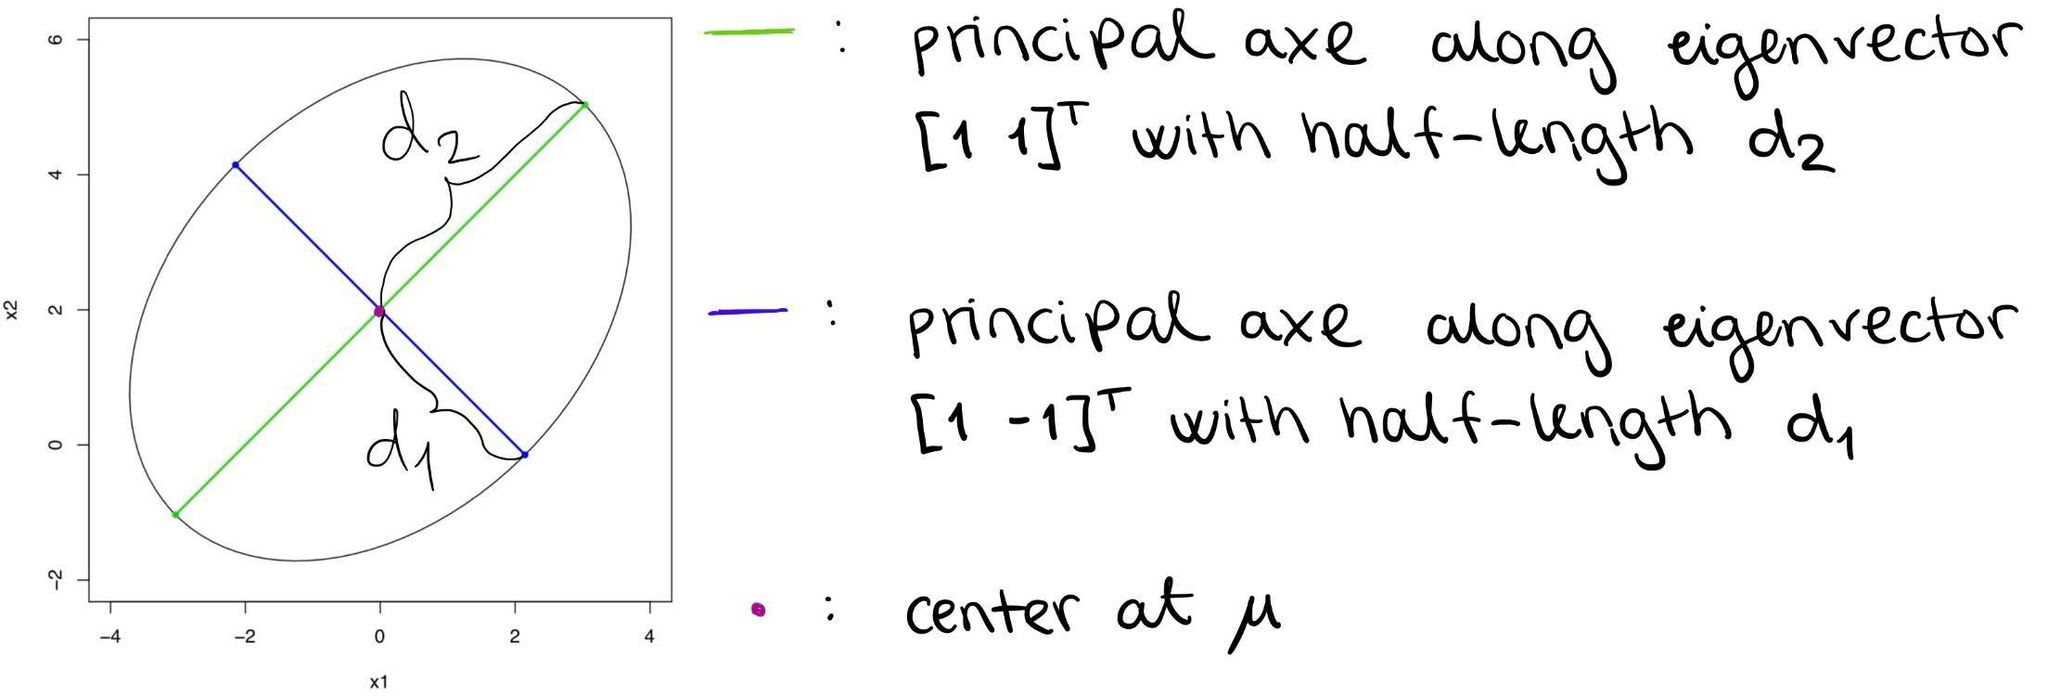
\includegraphics[width=1\textwidth]{figur1.jpg}
    \caption{}
    \label{figure}
\end{figure}